
\subsection{Getting the network} 

To get the data for our simulation, we used the so-called Facebook Graph API, a programming tool designed to support better access to conventions on the Facebook social media platform.\footnote{http://www.techopedia.com/definition/28984/facebook-graph-api} 
\\
Unfortunately, there is no implementation for Matlab, so we programmed the data-fechting in python. For the coding in python we used the facebook sdk\footnote{https://github.com/pythonforfacebook/facebook-sdk}. 

\paragraph{Get access}

First, one needs to get access to the social graph. Therefore, you need to enter an access token\footnote{https://developers.facebook.com/docs/facebook-login/access-tokens/}. 

\begin{lstlisting} 
token = raw_input('Enter your Access Token: ')
anonym = input('Do you want to anonymize your Data? Yes (1) or No (0)? ')
graph = facebook.GraphAPI(token)

\end{lstlisting}

\paragraph{Get graph}

Having enterd a valid token, we can now access all information this token provide us.  For simplicty, we'll only discuss  the non-anonymized case in details. [For more details on the anonymization, look at subsection anonymization]

\begin{lstlisting} 
profile = graph.get_object("me")
friends = graph.get_connections("me", "friends")
\end{lstlisting}

In our case, we're interested in data about our own profile, as well as all available information we get from our friends.
The object friends is nothing else but an array that contains all id's of our friends. For each id there is another array, named data, that contains all (available) information about this specific friend.  

\begin{lstlisting}
friend_list = [friend['id'] for friend in friends['data']]
\end{lstlisting}

With this simple for-loop, one can now get a list of all friends. Since we're not primarly interesseted in our friends, but the connection in between them, we have to access at least the mutualfriends. 

\begin{lstlisting}
mutualfriends = graph.get_connections(tfriend, "mutualfriends")
\end{lstlisting}

The object mutualfriends provides us a list with all mutualfriends of ''me'' and friend ''tfriend'' (which is nothing else but one of the id's we have in the saved in "friend\_list"

Repeat this proceedure for all friends, and we'll get exatly what we're looking for - a graph of all connection between our friends.

\paragraph{Get activity}

How did we define the parameter activity? We simply determine for each friend how many posts he makes on average per day. This gives us an indicator, how active a certain person is on facebook. 

Again, this is done fairly quickly (using graph api).

\begin{lstlisting}
statuses = graph.get_connections(tfriend, "statuses", fields="updated_time", limit="100")
\end{lstlisting}

This objecct provides us, all information we need (a list of all posts incl. a time stamp when it's been posted) to calculate the above mentioned quotient.

\paragraph{Get coordinates}
To visualise the network in MatLab, the software "Gephi" was used to determine the x- and y- coordinates of each individual. Therefore, the file "gephi.csv", an edge list of the network, was imported. The nodes were then arranged in communities using the layout method "ForceAtlas2". Finally, normalised node coordinates where exported to "coordinates.gdf". After deleting all headers and all edge data from this file, the coordinates could be easily imported to MatLab. The Network is visualized in Figure \ref{Network-Graph}.

\begin{figure}
\begin{center}
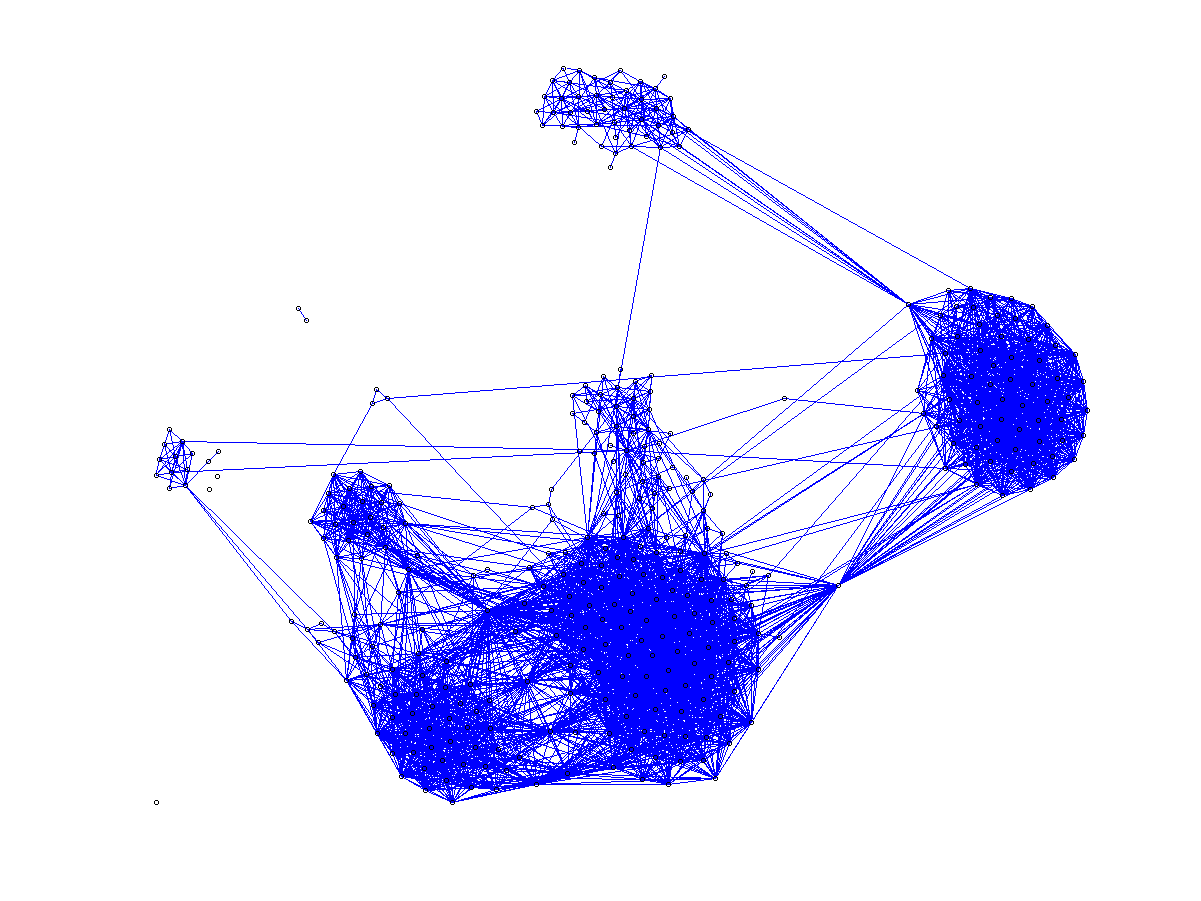
\includegraphics[width=7cm]{Network-Graph}
\caption{sdlhfa}
\label{Network-Graph}
\end{center}
\end{figure}

\paragraph{Anonymization}

The anonymization is acutally only a pseudo-anonymization. First all id's get arranged in order of size. Secondly, we create a list from 1 to n (number of friends). We then define a bijection between the two sets, such that the i-th element of the first set, maps to the i-th element of the second set. 

Eventhough, this is not really anonymizing our data. It is more then sufficient for our purpose. 




